\section{Resultater}

\subsection{M�linger i romtemperatur}

Figur \ref{fig:erbium_gammel} og \ref{fig:erbium_ny} viser Erbium referansepr�ve ved 300K, pumpet med 532nm laser, med grating lik 300.

%Erbium_gammel.eps
%Erbium_ny.eps

\begin{figure}[H]
\centering
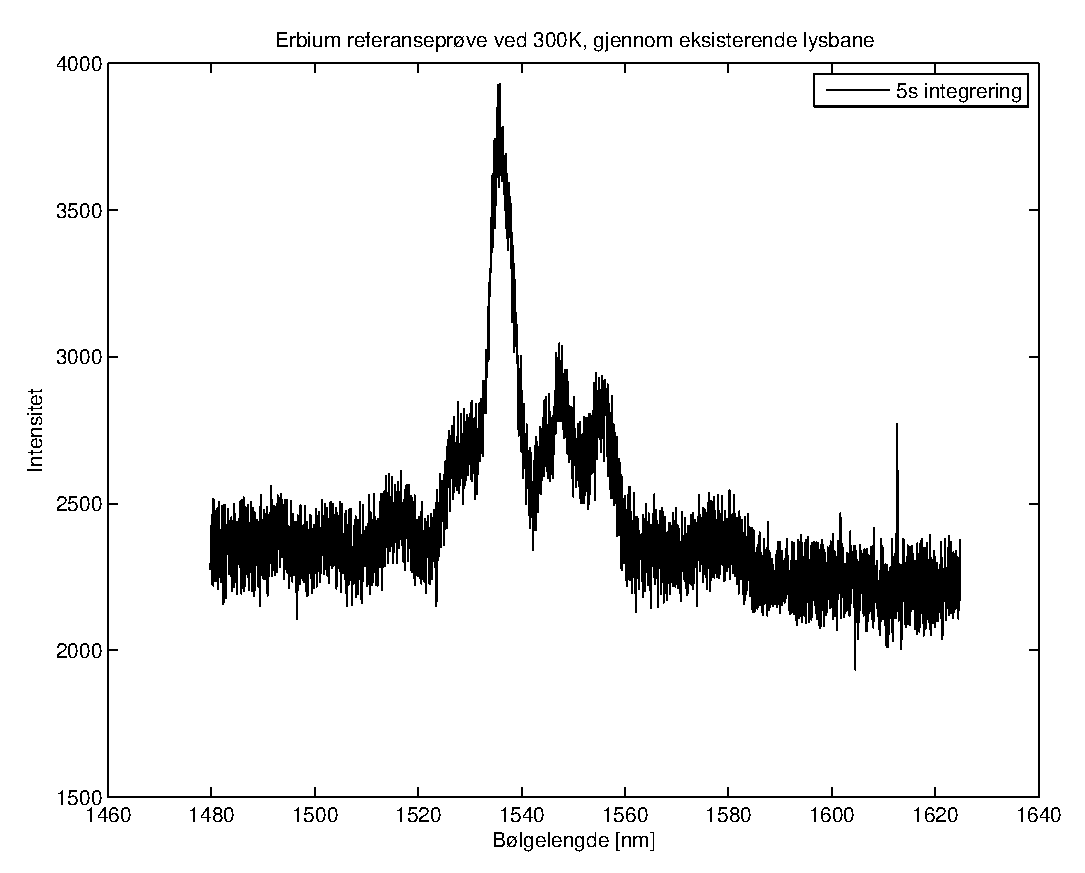
\includegraphics[scale=0.5]{Erbium_gammel.eps}
\caption{Eksitert lys sendt gjennom eksisterende laboppsett, med grating rundt 1550nm}%
\label{fig:erbium_gammel}%
\end{figure}

\begin{figure}[H]
\centering
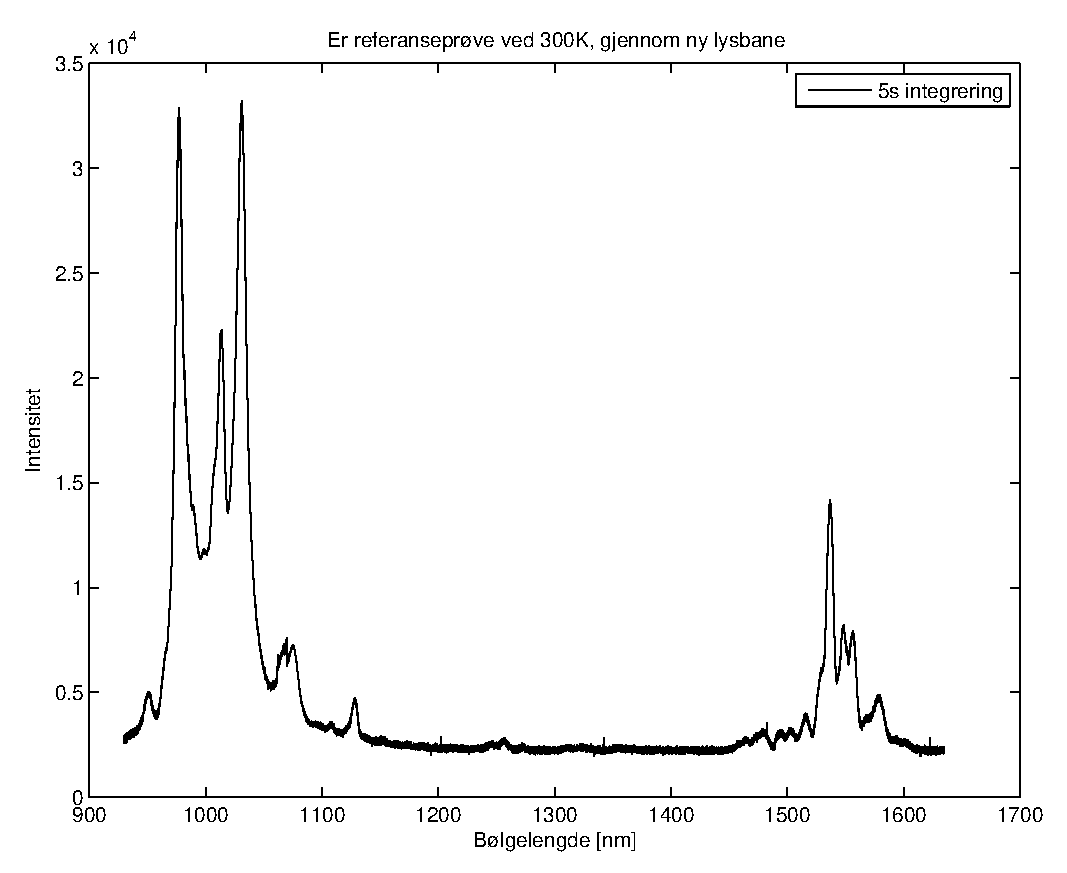
\includegraphics[scale=0.5]{Erbium_ny.eps}
\caption{Eksitert lys sendt gjennom nye komponenter}%
\label{fig:erbium_ny}%
\end{figure}

%Polert_300K.eps
%Upolert_300K.eps

Figur \ref{fig:polert_sample} og \ref{fig:upolert_sample} er m�linger gjort ved 300K, pumpelys lik 532nm, og grating lik 300. Den upolerte pr�ven er samme som i figur \ref{fig:cryolabtap}. Den andre pr�ven i figur \ref{fig:upolert_sample} er lik p� alle m�ter, bortsett fra at den er polert p� overflaten.

\begin{figure}[H]%
\centering
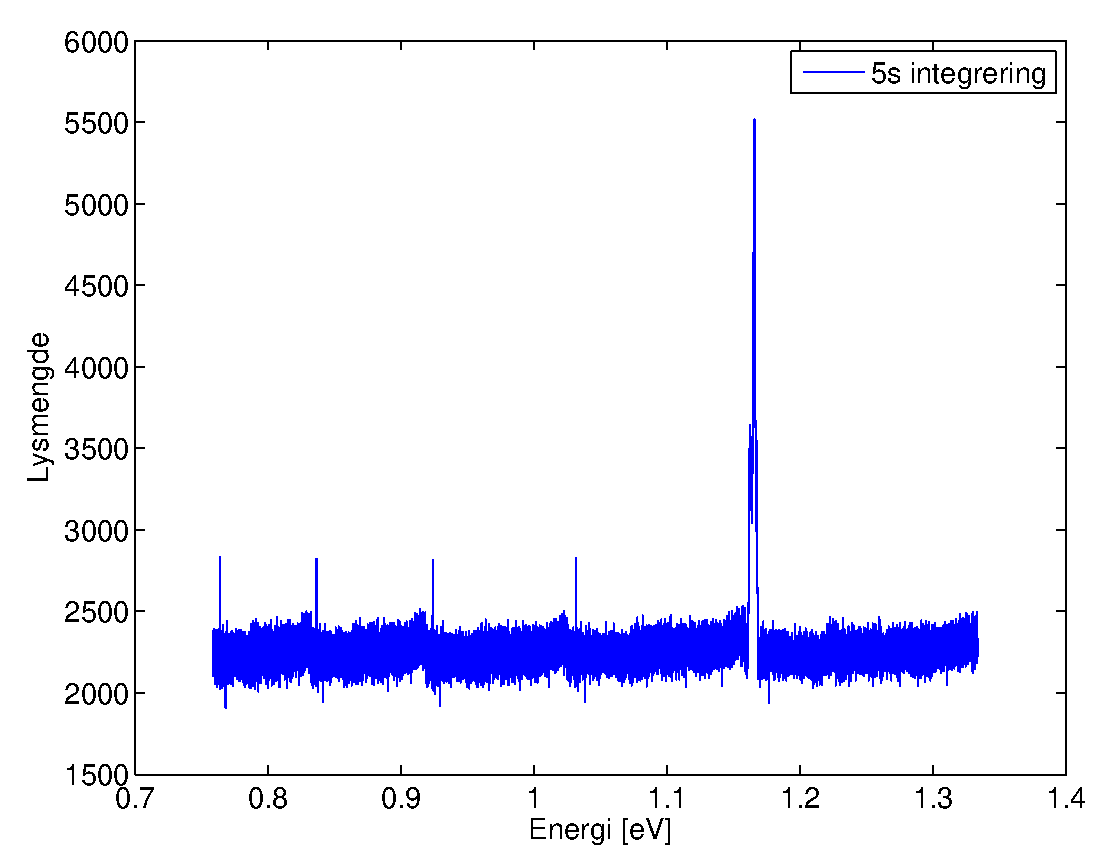
\includegraphics[scale=0.5]{Polert_300K.eps}
\caption{Polert multikrystallinsk silisium}%
\label{fig:upolert_sample}%
\end{figure}

\begin{figure}[H]%
\centering
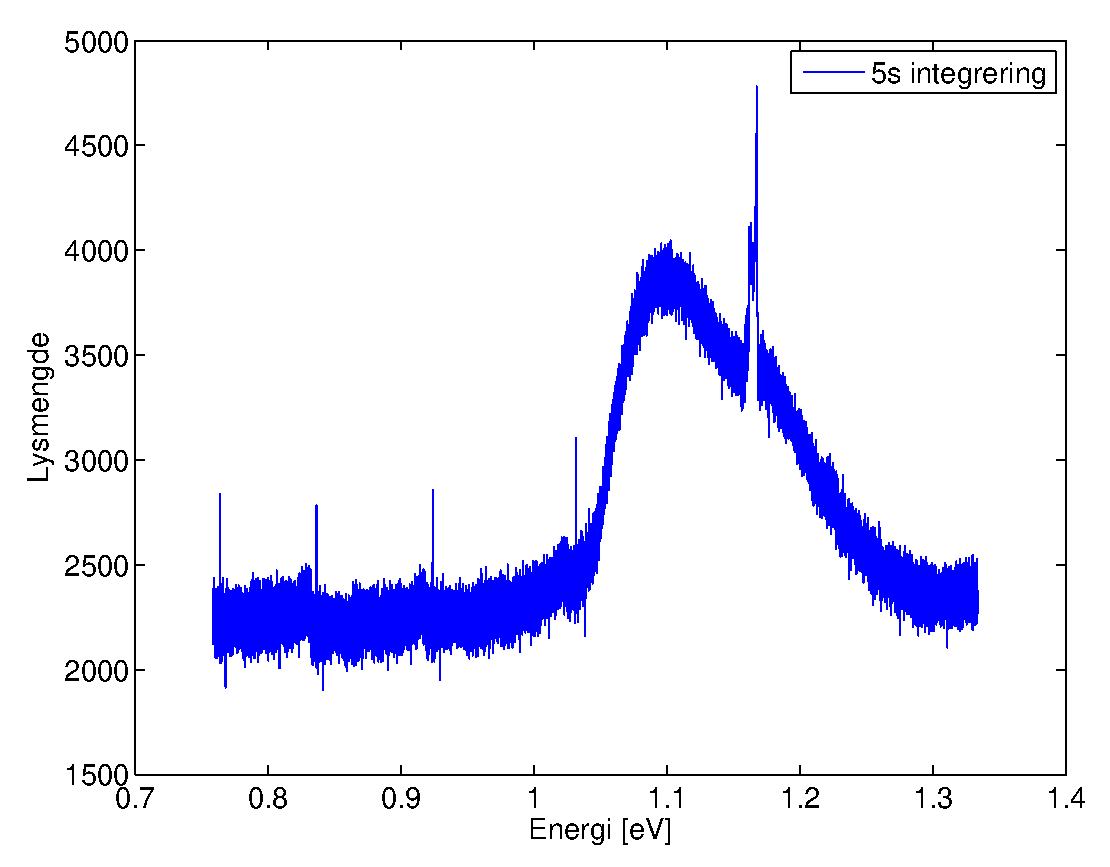
\includegraphics[scale=0.5]{Upolert_300K.eps}
\caption{Upolert multikrystallinsk silisium}%
\label{fig:polert_sample}%
\end{figure}


\subsection{M�linger ved lavtemperatur}

Grating er satt til 300, og pumpelyset er fortsatt 532nm. Resultatene i figur \ref{fig:sample_4_2_1} og \ref{fig:sample_4_2_2} viser til samme punkt p� pr�ven.

\begin{figure}[H]%Sample_4.eps
\centering
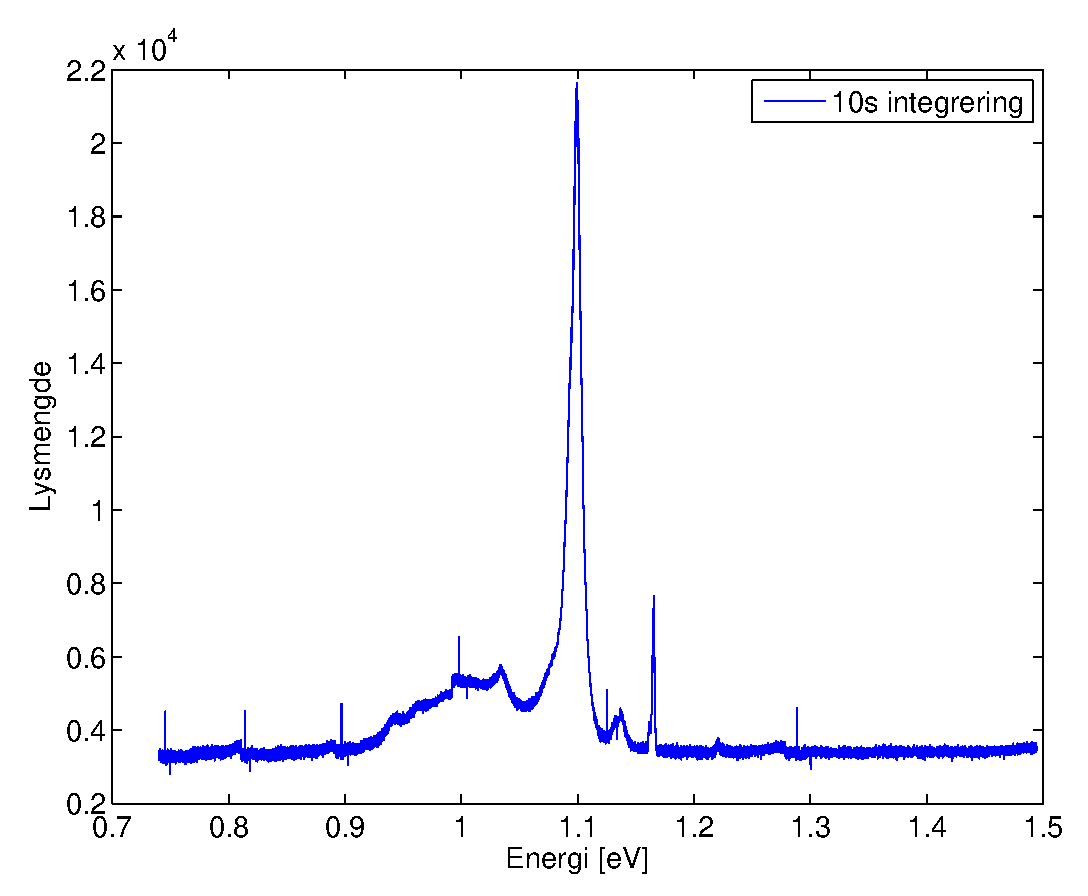
\includegraphics[scale=0.5]{Sample_4.eps}
\caption{Belyst med 13mW, ved 23K}%
\label{fig:sample_4_}%
\end{figure}

%Sample_4_1.eps
\begin{figure}[H]%
\centering
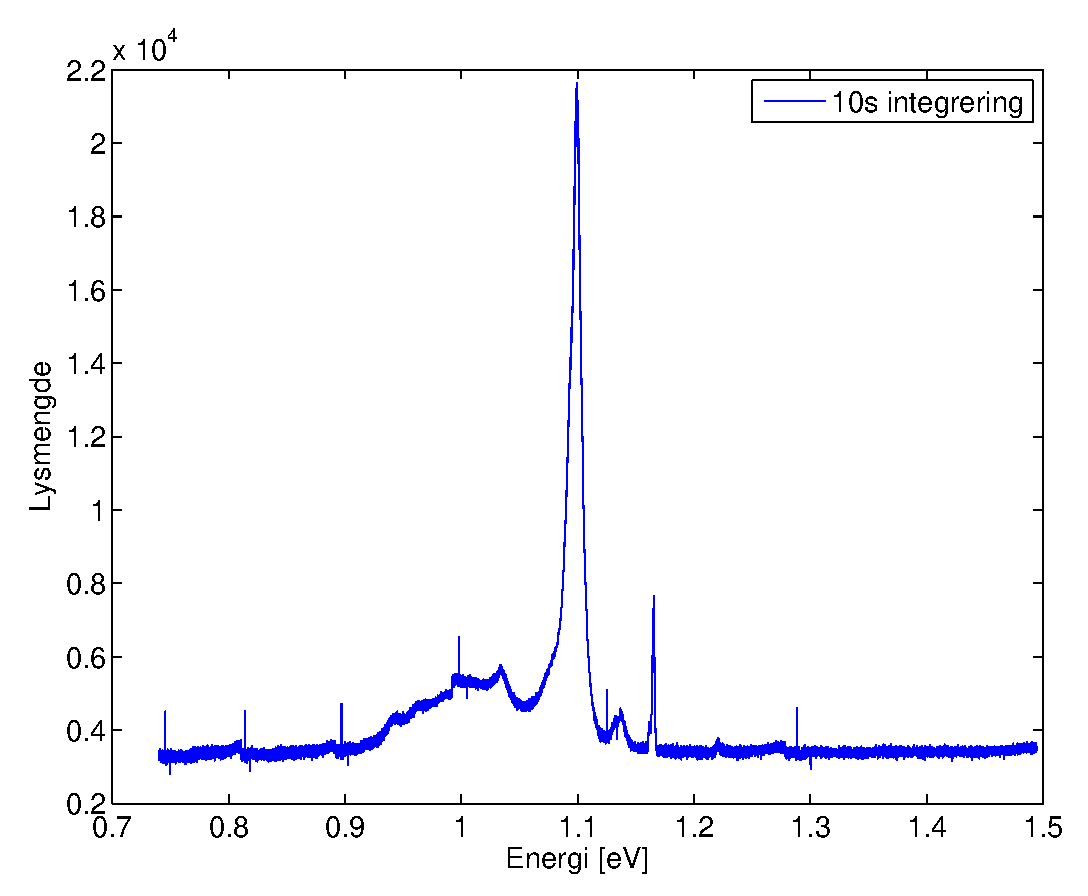
\includegraphics[scale=0.5]{Sample_4.eps}
\caption{Belyst med 4.6mW, ved 18K}%
\label{fig:sample_4_1}%
\end{figure}

%Sample_4_2_1.eps
\begin{figure}[H]%
\centering
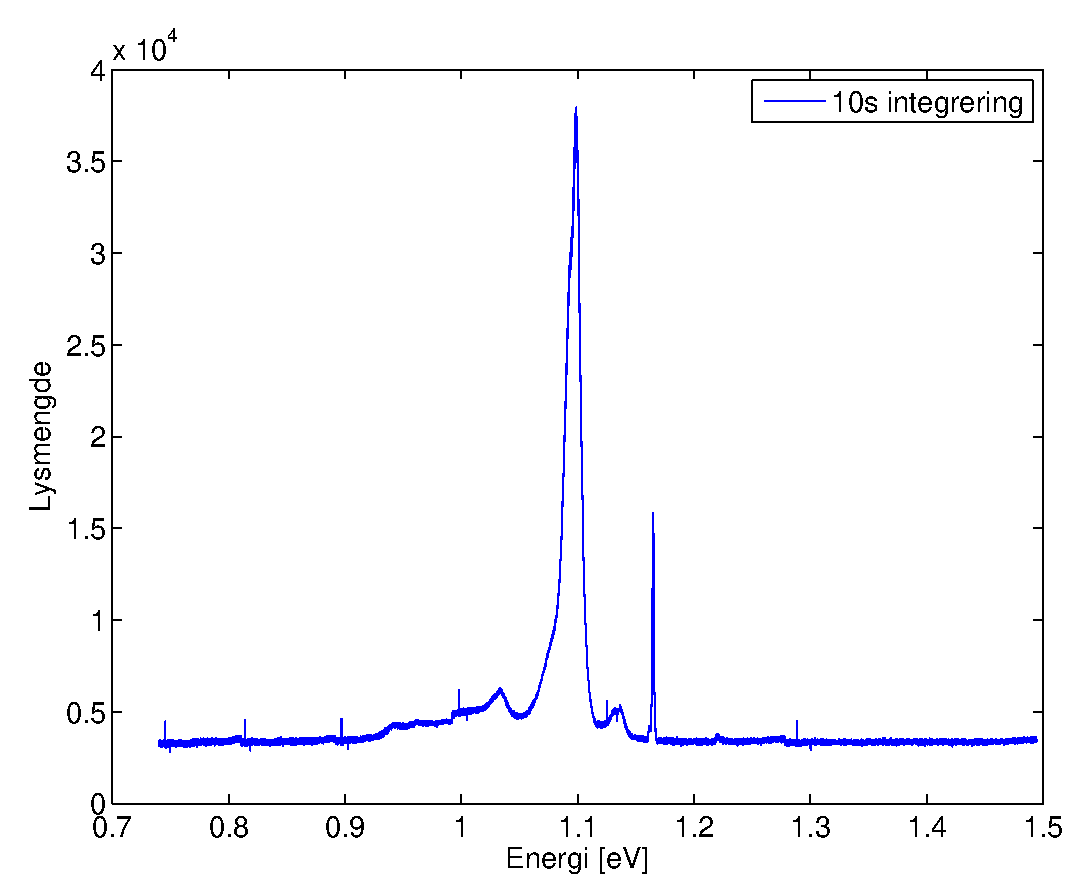
\includegraphics[scale=0.5]{Sample_4_2_1.eps}
\caption{Belyst med 15mW, ved 23K}%
\label{fig:sample_4_2_1}%
\end{figure}



\begin{figure}[H]%
\centering
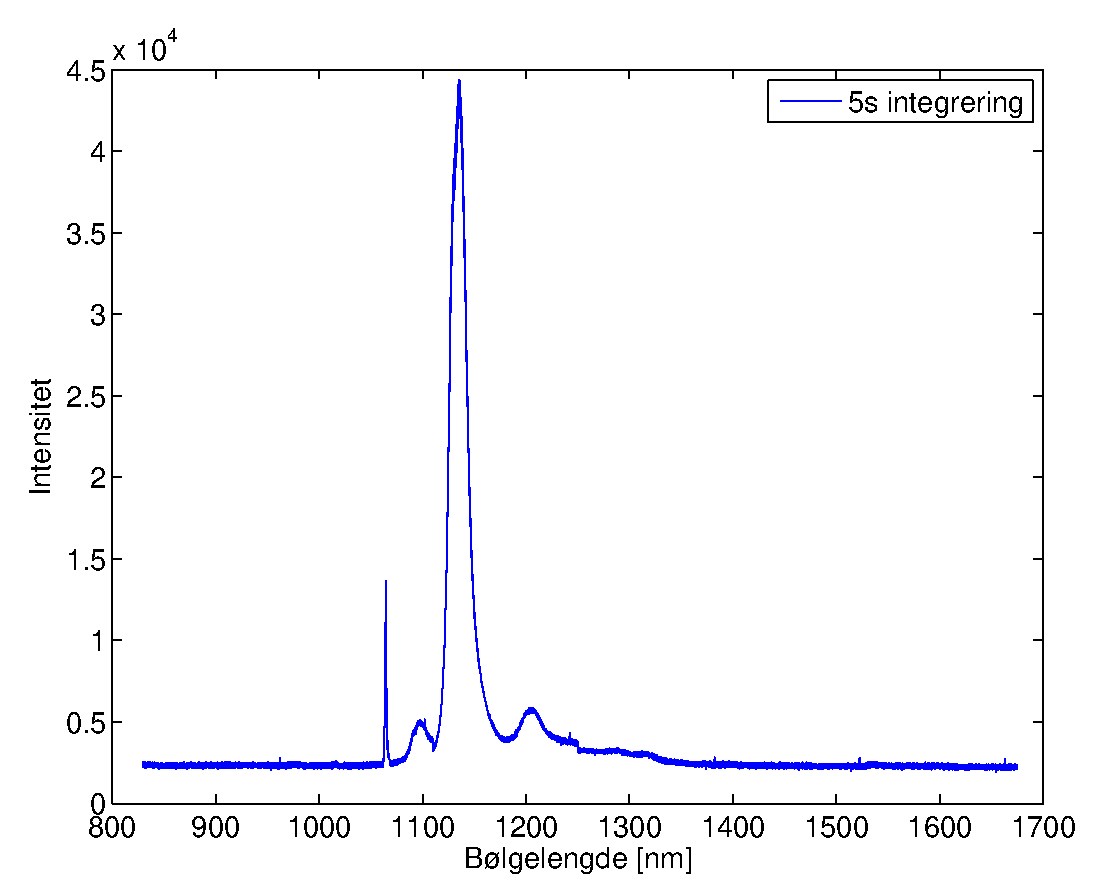
\includegraphics[scale=0.5]{Sample_4_2_2.eps}
\caption{Belyst med 30mW, ved 23K}%
\label{fig:sample_4_2_2}%
\end{figure}

%Posisjonsavhengighet.eps

\begin{figure}[H]%
\centering
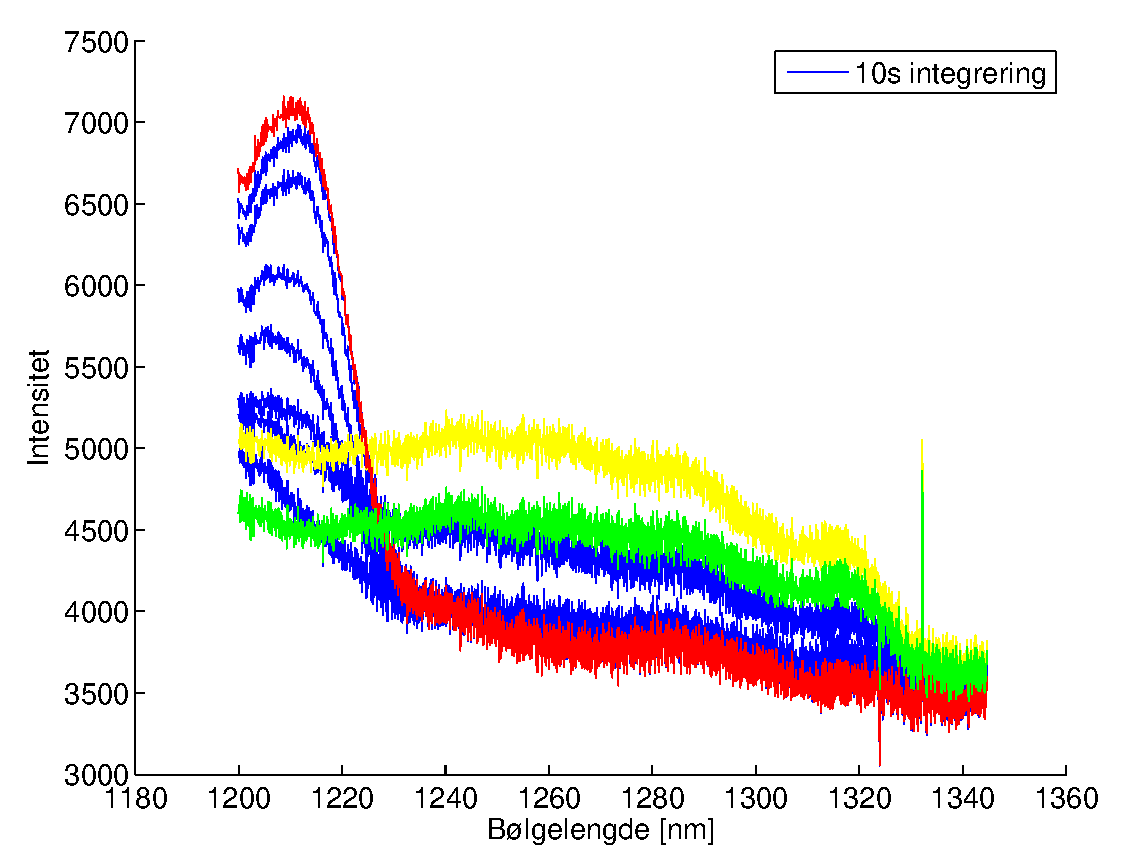
\includegraphics[scale=0.5]{Posisjonsavhengighet.eps}
\caption{Ulike posisjoner belyst med 13mW, ved 23K}%
\label{fig:posisjon}%
\end{figure}


% Sample4 bilde
\begin{figure}[H]%
\centering
	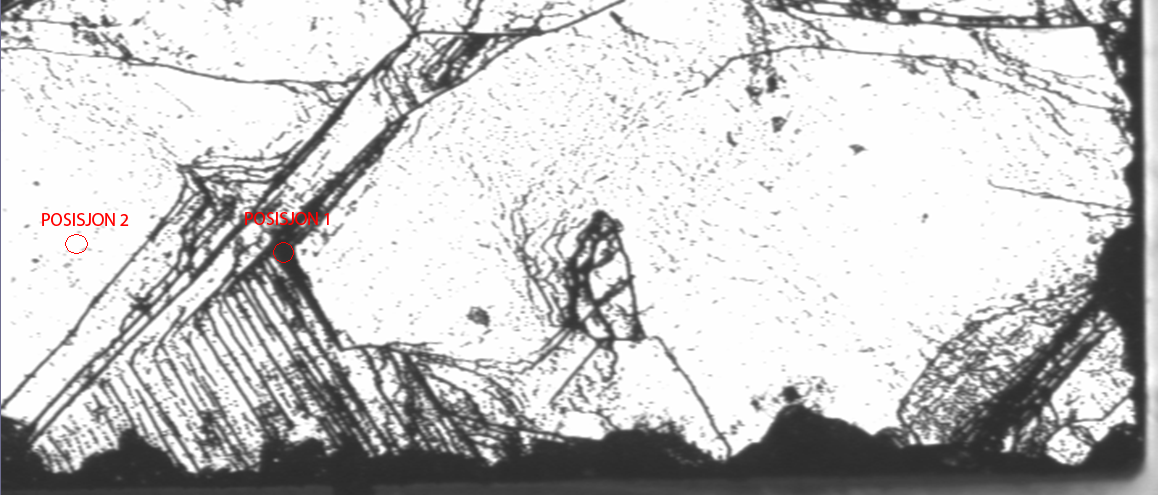
\includegraphics[width=15cm,bb=0 0 1158 495]{sample_4_edited.png}%
\caption{Posisjoner brukt for m�linger med lang integreringstid}%
\label{fig:sample4}%
\end{figure}


%Sample_4_SPOT_1_BAD.eps
\begin{figure}[H]%
\centering
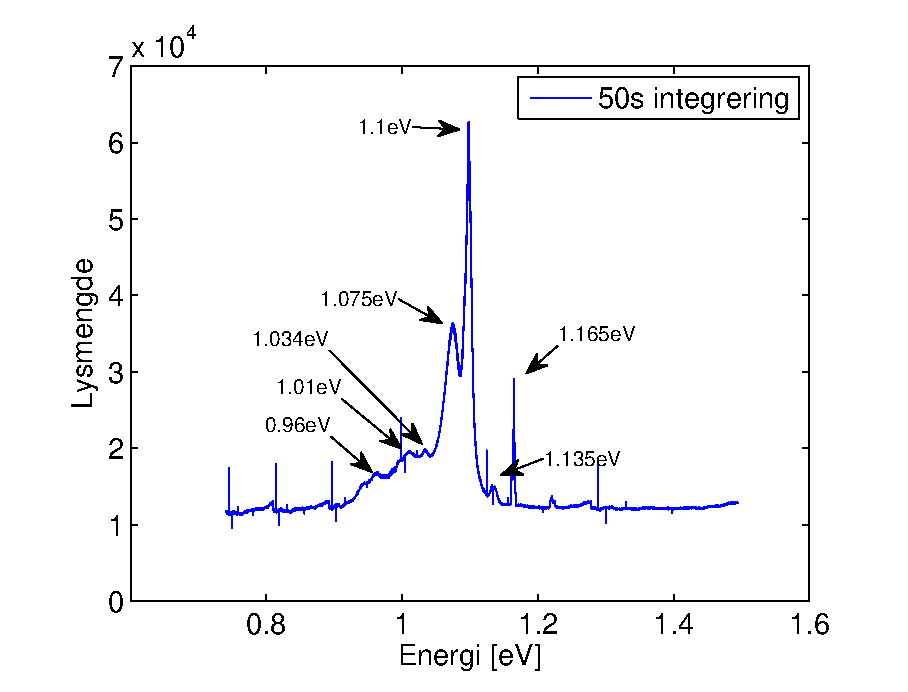
\includegraphics[scale=0.6]{Sample_4_SPOT_1_BAD.eps}
\caption{Resultatene fra posisjon 1 i figur \ref{fig:sample4}}%
\label{fig:spot1}%
\end{figure}

%Sample_4_SPOT_2_GOOD.eps
\begin{figure}[H]%
\centering
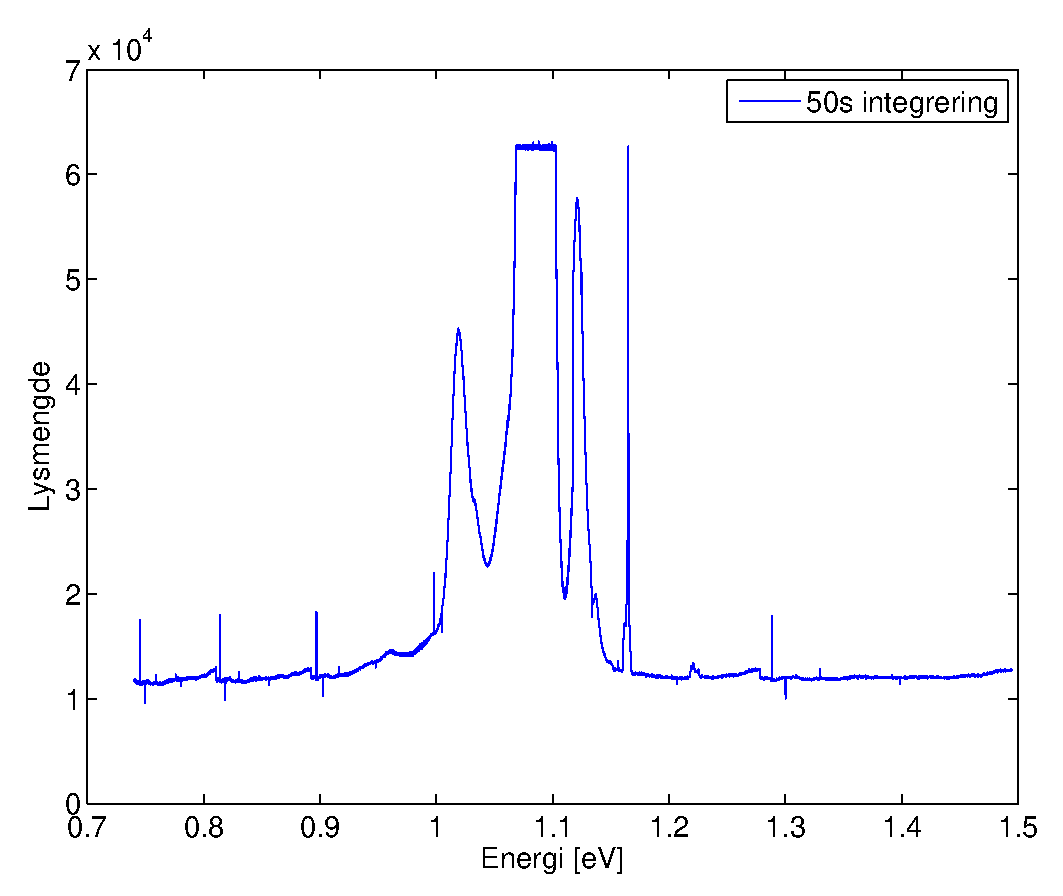
\includegraphics[scale=0.6]{Sample_4_SPOT_2_GOOD.eps}
\caption{Resultatene fra posisjon 2 i figur \ref{fig:sample4}}%
\label{fig:spot2}%
\end{figure}



